%\documentclass[compress,dvips,xcolor=table]{beamer}
\usepackage{etex}
%\documentclass{article}
%\usepackage{beamerarticle}
\usepackage{tikz}
\usetikzlibrary{shapes,arrows,positioning,calc,shadows,matrix,fit}
\usepackage{pgf-umlcd}
\tikzstyle{umlcolor}=[color=\umldrawcolor,fill=\umlfillcolor,text=\umltextcolor,drop shadow]
%\usepackage[turkish]{babel}
\usepackage[utf8]{inputenc}
\usepackage{listings}
\usepackage{multicol}
%\includeonlyframes{current}

\def\circtxt#1{$\mathalpha \bigcirc \mkern-13mu \mathtt #1$}

\mode<article>
{
  \usepackage{fullpage}
  \usepackage{pgf}
  \usepackage{hyperref}
}

\mode<presentation>
{
  \usetheme{metuceng}

%  \setbeamercovered{transparent}
}


\title{Programming Language Concepts}
\subtitle{Object Oriented Prog: Relations}
\author{Onur Tolga Şehitoğlu}
\institute[ODTÜ]{Bilgisayar Mühendisliği}
\subject{Object Oriented Prog: Relations}
\date{}
	\titlegraphic{\insertmetutitle\insertlicense}


\begin{document}
\lstset{language=C,
        basicstyle=\scriptsize\ttfamily,
        keywordstyle=\color{blue!50!black}\bfseries,
        identifierstyle=\color{blue!60!green}\sffamily,
        stringstyle=\color{red!70!green}\ttfamily,
	commentstyle=\color{blue!30!white}\itshape,
        showstringspaces=true}
\setbeamercolor{hexample}{bg=green!5!white,fg=black}%
\setbeamercolor{cexample}{bg=blue!5!white,fg=black}%
\setbeamercolor{pexample}{bg=orange!5!white,fg=black}%
\setbeamercolor{oexample}{bg=violet!5!white,fg=black}%

 \frame[plain]{\maketitle}

 \begin{frame}
 \frametitle{Outline}
 \begin{multicols}{2}
 \tableofcontents
 \end{multicols}
 \end{frame}


\section{Class Relations}
\begin{frame}
\frametitle{Class Relations}
\begin{columns}
\begin{column}{70mm}
\begin{itemize}
\item In Object Oriented  paradigm objects
interact in order to solve a problem.
\item Basic class relations:
\begin{itemize}
\item Aggragate (``has a'')
\item Composition (``has a'')
\item Generalization (inheritance, ``is a'')
\end{itemize}
\item Other associations/relations exist.
\item When two classes have such a relation, one \structure{depends} on
	the other.
\end{itemize}
\end{column}
\begin{column}{55mm}
\renewcommand{\umldrawcolor}{red!50!black}
\tiny
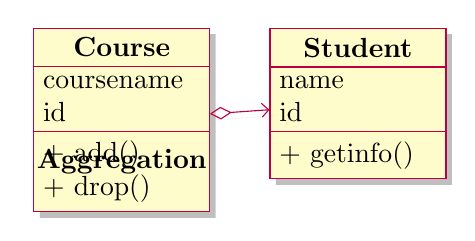
\begin{tikzpicture}
\begin{class}[text width=2cm]{Course}{0,0}
\attribute{coursename}
\attribute{id}
\operation{+ add()}
\operation{+ drop()}
\end{class}
\begin{class}[text width=2cm]{Student}{3cm,0}
\attribute{name}
\attribute{id}
\operation{+ getinfo()}
\end{class}
\aggregation{Course}{}{}{Student}
\node  at (0,-1.7cm) {\bf Aggregation};
\end{tikzpicture}\vspace*{1.5em}
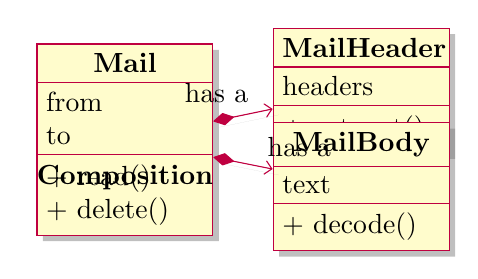
\begin{tikzpicture}
\begin{class}[text width=2cm]{Mail}{0,-0.2cm}
\attribute{from}
\attribute{to}
\operation{+ read()}
\operation{+ delete()}
\end{class}
\begin{class}[text width=2cm]{MailHeader}{3cm,0}
\attribute{headers}
\operation{+ getnext()}
\end{class}
\begin{class}[text width=2cm]{MailBody}{3cm,-1.2cm}
\attribute{text}
\operation{+ decode()}
\end{class}
\composition{Mail}{has a}{}{MailHeader}
\composition{Mail}{has a}{}{MailBody}
\node  at (0,-1.9cm) {\bf Composition};
\end{tikzpicture}\vspace*{1.5em}
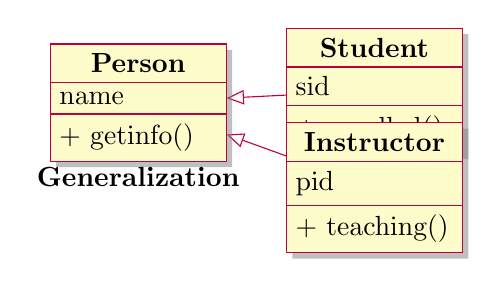
\begin{tikzpicture}
\begin{class}[text width=2cm]{Person}{0,-0.2cm}
\attribute{name}
\operation{+ getinfo()}
\end{class}
\begin{class}[text width=2cm]{Student}{3cm,0}
\inherit{Person}
\attribute{sid}
\operation{+ enrolled()}
\end{class}
\begin{class}[text width=2cm]{Instructor}{3cm,-1.2cm}
\inherit{Person}
\attribute{pid}
\operation{+ teaching()}
\end{class}
\node  at (0,-1.9cm) {\bf Generalization};
\end{tikzpicture}
%\tiny
%\rnode{course}
%{\umlClass{Course}{
%    coursename \\
%    id\\
%    \hline
%    add() \\
%    drop() \\
%}} \hspace*{4em} 
%\rnode{student}
%{\umlClass{Student}{
%    name\\
%    id\\
%    \hline
%    getinfo() \\
%}}
%\ncline{course}{student}
%\ncputicon{umlAgreg}\\
%Aggragate\\
%
%\rnode{mail}
%{\umlClass{Mail}{
%    from \\
%    to\\
%    \hline
%    read() \\
%    delete() \\
%}} \hspace*{4em} 
%\begin{minipage}[c]{2cm}
%\rnode{header}
%{\umlClass{MailHeader}{
%    headers\\
%    \hline
%    getnext() \\
%}}\\
%\rnode{body}
%{\umlClass{MailBody}{
%    text\\
%    \hline
%    decode() \\
%}}\end{minipage}
%\ncangle[angleB=180]{mail}{body}
%\ncputicon{umlCompos}
%\ncangle[angleB=180]{mail}{header}
%\ncputicon{\tiny umlCompos}\\
%Composition\\
%\rnode{person}
%{\umlClass{Person}{
%    name \\
%    \hline
%    getinfo() \\
%}} \hspace*{4em} 
%\begin{minipage}[c]{1.5cm}
%\rnode{istudent}
%{\umlClass{Student}{
%    id\\
%    \hline
%    getinfo() \\
%}}\\
%\rnode{instructor}
%{\umlClass{Instructor}{
%    pid\\
%    \hline
%    getinfo() \\
%}}
%\end{minipage}
%\ncangle[angleB=180]{person}{istudent}
%\ncputicon{umlHerit}
%\ncangle[angleB=180]{person}{instructor}
%\ncputicon{umlHerit}\\
%Generalization
\end{column}
\end{columns}
\end{frame}

\defverbatim[colored]\codeAggragate{
\begin{lstlisting}[language={C++},escapechar=\#]
class Course {
 char name[40];
 int no;
 List students;
public:
 void register(Student &a) {
   student.insert(&a);
 };
} ceng242 ;

void Student {
 char name[30];
 int no;
public:
 void add(Course &c) {
   c.register(*this);
 }
};
\end{lstlisting}}
\section{Aggragate}
\begin{frame}
\frametitle{Aggragate}
\begin{itemize}
\item Class A can have 0 or more instance of class B
\item Lifetime of class B objects are independent of class A
\item Catalog relationship. In terms of \structure{references}. 
\item Members of class B are regular objects in scope of A\\
\alert{they are not in scope of A}. So private members ... ?
\end{itemize}
\noindent
\begin{beamercolorbox}{cexample}
\begin{multicols}{2}[\columnseprule=.5pt]
\codeAggragate
\end{multicols}
\end{beamercolorbox}
\end{frame}

\defverbatim[colored]\codeCompose{
\begin{lstlisting}[language={C++},escapechar=\#]
class FrameBox {
 Shape frame;
 String text;
 double coordx,coordy;
public:
 Framebox(Frame &f, 
          String &t) {
  ...}
  void draw() { 
    frame.draw(); text.draw();
} ceng242 ;

class Shape {
 enum Type {Circle,Rect} type;
 double sizex, sizey;
public:
 void draw();
};

class String {
...
};
\end{lstlisting}}
\section{Composition}
\begin{frame}
\frametitle{Composition}
\begin{itemize}
\item Class A can have 0 or more instance of class B
\item Lifetimes of class B objects depend on the class A object
\item Class B objects are destroyed when A is destroyed.
\item Members of class B are regular objects in scope of A\\
\alert{they are not in scope of A} as in aggragate.
\end{itemize}
\noindent
\begin{beamercolorbox}{cexample}
\begin{multicols}{2}[\columnseprule=.5pt]
\codeCompose
\end{multicols}
\end{beamercolorbox}
\end{frame}

\begin{frame}
\tiny
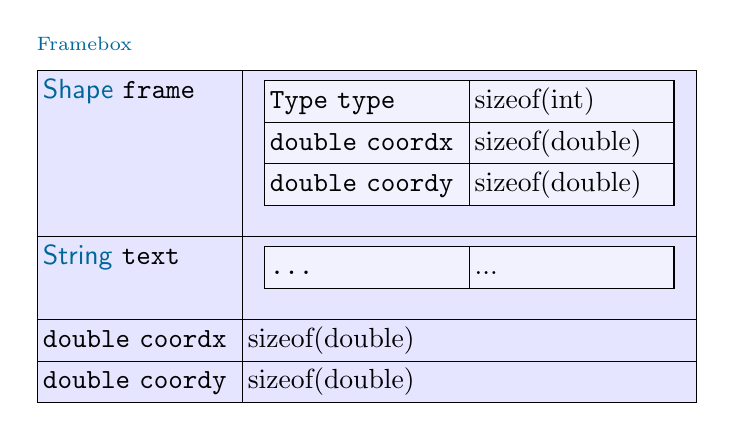
\begin{tikzpicture} [class/.style={matrix of nodes, row sep=-\pgflinewidth, column sep=-\pgflinewidth,
		 nodes={align=left,rectangle,draw=black,inner xsep=2pt, inner ysep=0pt, outer sep=0pt,text height=1em,fill=blue!10!white },
		 nodes in empty cells, ampersand replacement=\&}]
\matrix [class, 
		 column 1/.style = { text width=7em},
		 column 2/.style = { text width=16em},
		 row 1/.style = { text depth=5em},
		 row 2/.style = { text depth=2em},
		 row 3/.style = { text depth=.5em},
		 row 4/.style = { text depth=.5em},
	] (frame) {
\tt {\color{blue!60!green}\sf Shape} frame\&  \\
\tt {\color{blue!60!green}\sf String} text\&	\\
\tt double coordx\&	sizeof(double)\\
\tt double coordy\&	sizeof(double)\\
} node [above=6pt of frame.north west,blue!60!green,anchor=west] {\scriptsize Framebox};
\matrix [class,below=0pt of frame-1-2.north,
		 text depth=.5em, nodes={fill=blue!5!white},
		 column 1/.style = { text width=7em},
		 column 2/.style = { text width=7em}
] {
		\tt Type type \& sizeof(int) \\ 
		\tt double coordx \& sizeof(double) \\
		\tt double coordy \& sizeof(double) \\ };
\matrix [class,below=0pt of frame-2-2.north,
		 text depth=.5em,nodes={fill=blue!5!white},
		 column 1/.style = { text width=7em},
		 column 2/.style = { text width=7em}
] {
		\tt ... \& ... \\ 
};
\end{tikzpicture}
\normalsize
\begin{itemize}
\item Container class vs. contained classes
\item Composition nests storage of contained classes into container class.
\item \texttt{frame} and \texttt{text} are regular object variables in
member functions of \texttt{Framebox}
\item Integrity of contained objects?
\end{itemize}
\end{frame}

\defverbatim[colored]\codeCompExp{
\begin{lstlisting}[language={C++},escapechar=\#]
class Student {
 char name[40];
 int id;
public:
 Student() { name[0]=0; id=0;}
 void setnameid(const char *s,int i);
 ...
};

class StudentArr {
  Student *content;
public:
  StudentArr(int size) {
      content=new Student[size];
  }
  ~StudentArr() { delete [] content;}
  Student &operator[](int i) {
      return content[i];
  }
}
...
StudentArr a(10);
a[5].setnameid("onur",55717);
\end{lstlisting}}
\begin{frame}
\begin{beamercolorbox}{cexample}
\codeCompExp
\end{beamercolorbox}
\end{frame}

\defverbatim[colored]\codeCompCons{
\begin{lstlisting}[language={C++},escapechar=\#]
class A {
  int x;
public:
  A(int a) { x=a;}
};
class B {
  int y;
public:
  B(int a) { y=a;}
};
class C {
  int c;
  A a;
  B b;
public:
  C(int x,y,z)#\color{red!50!black}\sf :a(x),b(y)# { 
      c=z; /*can refer a,b */ 
  }
  ~C() { /*can refer a,b */}
};
\end{lstlisting}}
\subsection{Integrity of Contained Objects}
\begin{frame}
\frametitle{Integrity of Contained Objects}
\begin{beamercolorbox}{cexample} \begin{multicols}{2}[\columnseprule=.5pt]
\codeCompCons \end{multicols}
\end{beamercolorbox}
\begin{itemize}
\item When constructors called? Tip: Container class constructor may refer to the contained
objects.
\item When destructors called? Tip: Container class destructor may refer to the contained
objects.
\end{itemize}
\end{frame}

\begin{frame}
\begin{itemize}
\item Constructors of contained objects called just before the body of container constructor
executed.
\item Destructors of contained objects called just after the container destructor called.
\item Container constructor can pass arguments to member object constructors.\\
	\lstinline!ACons(int x):a(x),b(x),c(x) \{...\}!
\item \lstinline!friend! declaration can be used if the objects need to access others private
member.
\end{itemize}
\end{frame}

\defverbatim[colored]\codeInher{
\begin{lstlisting}[language={C++},escapechar=\#]
class Shape {
 double x,y;
public:
 Shape(double a, double b);
 void draw();
};

class Circle: #\color{red!70!black}public Shape# {
 double radius;
public:
 void draw();
};

class Square: #\color{red!70!black}public Shape# {
 double width;
public:
 void draw();
};
\end{lstlisting}}
\section{Generalization/Inheritance}
\begin{frame}
\frametitle{Generalization/Inheritance}
\begin{itemize}
\item Class \lstinline!Circle! \alert{is a} \lstinline!Shape! but
	has extra features.
\item It has all members of \lstinline!Shape! plus specific
	ones.
\item \lstinline!Circle! extends \lstinline!Shape!
\item \lstinline!Shape! is super class of \lstinline!Circle!
\item \lstinline!Shape! is more general, \lstinline!Circle! has
	more information
\end{itemize}
\noindent
\begin{beamercolorbox}{cexample}
\begin{multicols}{2}[\columnseprule=.5pt]
\codeInher
\end{multicols}
\end{beamercolorbox}
\end{frame}

\newcommand{\rnode}[1]{}
\begin{frame}
\scriptsize
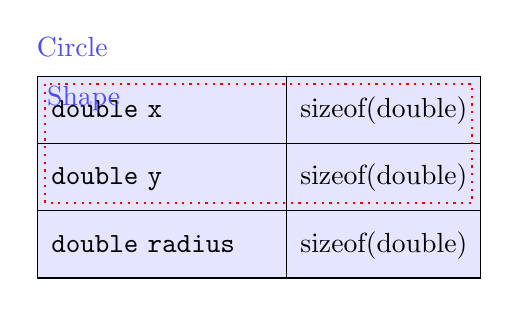
\begin{tikzpicture}
\matrix [matrix of nodes, row sep=-\pgflinewidth, column sep=-\pgflinewidth,
		 nodes={rectangle,draw=black,inner sep=5pt, outer sep=0pt,text height=10pt,text depth=1ex,
				fill=blue!10!white},
		 column 1/.style = { text width=8em},
		 column 2/.style = { text width=6em},
		 nodes in empty cells, ampersand replacement=\&] (circ) {
\tt double x\&	sizeof(double)\\
\tt double y\&	sizeof(double)\\
\tt double radius\&	sizeof(double)\\
} node[above=0mm of circ.north west,anchor=south west,blue!70!white] {\normalsize Circle};
\draw [draw=red,dotted,thick] ($(circ-1-1.north west) + (1mm,-1mm)$) rectangle ($(circ-2-2.south east) + (-1mm,1mm)$) ;
\node [anchor=north west, blue!70!white] at (circ-1-1.north west) {\normalsize Shape};
\end{tikzpicture}
\begin{itemize}
\item There is an inherent \lstinline!Shape! object in each \lstinline!Circle! object.
\item Env(\lstinline!Circle!) = Env(\lstinline!Shape!) $ \cup $ Members specific
	to \lstinline!Circle!
\item All members are inherited. They \alert{are} in the scope of the subclass.
\item How about their accessibility, protection?
\item Two new thing: \structure{protected} label, \structure{derivation label} 
\item A subclass can access \structure{protected} members of the upper classes.
\item \structure{derivation label} is a filter defining how members of superclass
	interpreted when used through subclass (object of subclass or further derivations from
	subclass)
\end{itemize}
\end{frame}

\defverbatim[colored]\codeInherAcc{
\begin{lstlisting}[language={C++},escapechar=\#]
class A {
private:   int a;
protected: int b;
public:    int c;
   void Amember() { #\circtxt{1}# }
} Aobj ;
class B: #\alert{DLABEL}  A# { // DLABEL=public|protected|private 
   void Bmember() { #\circtxt{2}# };
} Bobj;
... Aobj.#\circtxt{3}# ;
... Bobj.#\circtxt{4}# ;
class C: public B {   
    void Cmember() { #\circtxt{5}# } };
\end{lstlisting}}
\begin{frame}
\begin{beamercolorbox}{cexample}
\codeInherAcc
\end{beamercolorbox}

\newcommand{\ATOK}{\only<2->{\color{green!30!black}{$\surd$}}}
\newcommand{\ATNO}{\only<2->{\color{red!30!black}{$\times$}}}
{\scriptsize
\begin{tabular}[t]{>{\tt}l|lll}
  & \circtxt{1} & \circtxt{2} & \circtxt{3} \\ \hline
a & \ATOK  & \ATNO & \ATNO \\
b & \ATOK & \ATOK & \ATNO \\
c & \ATOK & \ATOK & \ATOK  \\
\end{tabular} \hfill
\begin{tabular}[t]{>{\tt}l|lll|lll}
          & \multicolumn{3}{c|}{\circtxt{4}}  &
	   \multicolumn{3}{c}{\circtxt{5}} \\
	  	\cline{2-7}
\alert{\tt DLABEL}  &  \tt a & \tt b & \tt c & \tt a & \tt b & \tt c \\ \hline
private   &  \ATNO & \ATNO & \ATNO & \ATNO & \ATNO & \ATNO \\
protected & \ATNO & \ATNO & \ATNO & \ATNO & \ATOK & \ATOK \\
public    &  \ATNO & \ATNO & \ATOK & \ATNO & \ATOK & \ATOK \\
\end{tabular}
}
\begin{itemize}
\item \structure{\tt DLABEL} is only significant outside of the derived class
\item protection is minimum of original label and \structure{\tt DLABEL}
\end{itemize}
\end{frame}

\defverbatim[colored]\codeInhCons{
\begin{lstlisting}[language={C++},escapechar=\#]
class A {
  int x;
public:
  A(int a) { x=a;}
  ~A() { ... }
};
class B : public A {
  int y;
public:
  B(int a)#\color{red!50!black}\sf :A(a)# { y=a;}
  ~B() { ... }
};
\end{lstlisting}}
\subsection{Integrity of Superclass}
\begin{frame}
\begin{itemize}
\item The inherent superclass object should have a valid value.
\item Constructors/Destructors should be called
\begin{beamercolorbox}{cexample}
\codeInhCons
\end{beamercolorbox}
\item Similar to contained objects:\\
	Superclass constructor called just before class constructor\\
	Superclass destructor called just after class destructor\\
\end{itemize}
\end{frame}

\defverbatim[colored]\codeInhHide{
\begin{lstlisting}[language={C++},escapechar=\#]
class A {
protected:
  int x;
public:
  int get() {return x};
} Aobj;
class B : public A {
  int x;
public:
  int get() {return x+#\alert{\sf A::x}#}
} Bobj;
...
cout << Bobj.get() << #\alert{\sf Bobj.A::get()}# ;
\end{lstlisting}}
\subsection{Member Hiding}
\begin{frame}
\frametitle{Member Hiding}
\begin{itemize}
\item members of the subclass hides member of the superclass with same name
\item but superclass member still exists
\item Scope operator can be used to access the member
\begin{beamercolorbox}{cexample}
\codeInhHide
\end{beamercolorbox}
\end{itemize}
\end{frame}

\section{Multiple Inheritance}
\begin{frame}
\frametitle{Multiple Inheritance}
\begin{itemize}[<+->]
\item Can a class be derived from two superclasses?
\item Land vehicle+Water vehicle $\rightarrow$ Hoovercraft
\item Student+Instructor $\rightarrow$ A lecturer still having PhD
\item A class hierarchy for vehicle types, a class hierarchy for engines:\\
	A boat with diesel engine, a car with electrical engine or hybrid engine
\item Multiple inheritance is necessary in some rare cases. C++ provides it,
	Java avoids it and uses \structure{Interfaces} for essential functionality similar to
	multiple inheritance.
\end{itemize}
\end{frame}

\defverbatim[colored]\codeMultInh{
\begin{lstlisting}[language={C++},basicstyle=\scriptsize\sf,escapechar=\#]
class Shape {
  int x,y;
public:
  Shape(int a, int b) { x=a; y=b;}
  ~Shape() { ... }
};
enum LineStyle {None, Solid, Dashed, Dotted, Double}
enum FillStyle {None, Full, Half, Pattern}
class ShapeAttr {
  LineStyle ls; double lw; FillStyle fill;
public:
  ShapeAttr(LineStyle a, double b, FillStyle c) { 
  	ls=a;lw=b;fill=c;}
  ~ShapeAttr() { ... }
};

class Circle: public Shape, public ShapeAttr {
  int radius;
public:
  Circle(int a, int b, int c, LineStyle d, 
     double e, FillStyle f):Shape(a,b),ShapeAttr(d,e,f) {
         radius=c;
  }
}
\end{lstlisting}}
\begin{frame}
\begin{beamercolorbox}{cexample}
\codeMultInh
\end{beamercolorbox}
\end{frame}

\subsection{Virtual base class}
\begin{frame}
\frametitle{Diamond Problem}
\begin{columns}
\begin{column}{.55\linewidth}
\begin{itemize}[<+->]
\item Multiple inheritance may cause same super class duplicated in the resulting class
\item Causes ambiguity.\\
	\lstinline!StudInst! contains two \lstinline!Person!'s\\
	\lstinline!get()! call refers to which one?\\
	What's the \lstinline!name! ?
\item Ambiguity can be solved by scope operator:\\
	\lstinline!Student::name! vs \lstinline!Instructor::name!
\item But a person with two names? Do we need that redundancy? \alert{NO!}

\end{itemize}
\end{column}
\begin{column}{.45\linewidth}
{\scriptsize
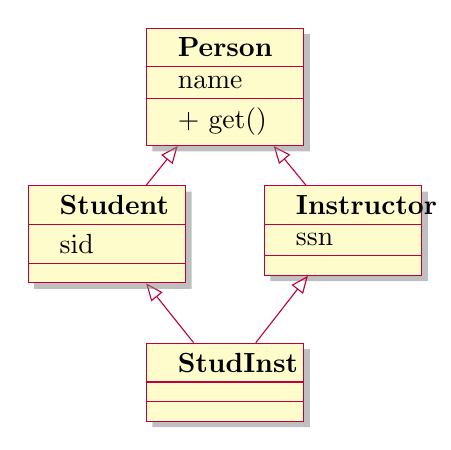
\begin{tikzpicture}
\begin{class}[text width=12mm]{Person}{0,0}
\attribute{name}
\operation{+ get()}
\end{class}
\begin{class}[text width=12mm]{Student}{-15mm,-2cm}
\inherit{Person}
\attribute{sid}
\operation{}
\end{class}
\begin{class}[text width=12mm]{Instructor}{15mm,-2cm}
\inherit{Person}
\attribute{ssn}
\operation{}
\end{class}
\begin{class}[text width=12mm]{StudInst}{0,-4cm}
\inherit{Student}
\attribute{}
\operation{}
\end{class}
\draw [umlcd style inherit line] (Instructor) -- (StudInst);
\end{tikzpicture}
}
\end{column}
\end{columns}
\end{frame}

\defverbatim[colored]\codeMultVirt{
\begin{lstlisting}[language={C++},escapechar=\#]
class Person {
        char name[40];
public: Person(char *s) {...}
};
class Student: virtual Person {
        int id;
public: Student(char *s, int i):Person(s) {...}
};
class Instructor: virtual Person {
        int ssn;
public: Instructor(char *s, int i):Person(s) {...}
};
class StudInst:public Student, public Instructor {
public: StudInst(char *s, int a, int b)
  	 :Person(s),Student(s,a),Instructor(s,b) {...}
};
\end{lstlisting}}
\begin{frame}
\frametitle{Virtual base class}
\begin{itemize}
\item \lstinline!virtual! keyword used in inheritance gets only a single 
	copy of base class in subclasses.
\begin{beamercolorbox}{cexample}
\codeMultVirt
\end{beamercolorbox}
\end{itemize}
\end{frame}

\begin{frame}
\begin{itemize}
\item \lstinline!virtual! keyword is for subclasses
\item It is an overloaded keyword. We also have virtual member
	functions which is completely different.
\item Multiple inheritence is not essential feature in OOP.
\item There are ways to live without it. Assume two hierarchies with
	M and N classes. First is under \lstinline!Vehicle!, second
	is \lstinline!Engine!
\item \structure{Bridge pattern} Put a \lstinline!Engine*!
	member in \lstinline!Vehicle!
\item \structure{Nested classes} Create all M$\times$N possibilities
	derived from \lstinline!Vehicle!
\item Such cases are rare and primary advantage of inheritance is 
\structure{Polymorphism}
\end{itemize}
\end{frame}
\end{document}


%\newcommand{\drawvehicle}{%
%\umlClass{Vehicle}{
%    capacity\\
%\hline
%    move() \\
%}}
%\newcommand{\drawland}{%
%\umlClass{Land}{
%    maxspeed\\
%\hline
%    \  \\
%}}
%\newcommand{\drawair}{%
%\umlClass{Aircraft}{
%    maxalt \\
%\hline
%    fly() \\
%}}
%\newcommand{\drawboat}{%
%\umlClass{Boat}{
%    class \\
%\hline
%    float() \\
%}}
%\newcommand{\drawcar}{%
%\umlClass{Car}{
%    class \\
%\hline
%    \\
%}}
%\newcommand{\drawtruck}{%
%\umlClass{Truck}{
%    class \\
%\hline
%    \\
%}}
%
%\begin{frame}
%\begin{tabular}{}
%\end{frame}

